% Appendix. Fragment, \input by spacenav.tex inside \appendix.
\section{The episode clock}
\label{app:clock}

Section~\ref{sec:clock} states the position that time is the least
interesting of the constraints a level places on a craft and the one most
easily mistaken for difficulty; this appendix collects the measurements
behind it. It is a position more than a finding, since deadlines and launch
windows are real constraints in the trajectory-design sources cited in
Section~\ref{sec:field}.
Fuel is a harder constraint, because it is consumed and cannot be recovered,
and exposure is the most interesting, because radiation, debris and
atmosphere each have their own geometry and dynamics and because avoiding
them shapes a route in ways the gravity alone would not. The clock, by
contrast, mostly penalizes a craft that chooses an energy-efficient path over
a fast one, which is the choice every mission in Section~\ref{sec:field} was
judged on.

The evidence that the 150\,s clock of this environment is binding in that
way comes from the optimizer of Section~\ref{sec:optimizer} flown on 32
two-target levels at four clocks, with control resolution held at 3.1\,s per
segment so that a longer clock buys more segments rather than coarser ones
(Figure~\ref{fig:clock}). Arrivals rise from $5/32$ at 150\,s to $8/32$ at
300\,s and $13/32$ at 600\,s, then fall back to $11/32$ at 900\,s; timeouts
fall monotonically from 18 to 5; and crashes, destructions and escapes go
from 9 at the shortest clock to 16 at the longest, though not
monotonically, so that of the thirteen timeouts a longer clock removes,
about half become arrivals and half become hazard endings. Thus, for the
optimizer at 150\,s, a substantial fraction of what the environment scores
as failure is the clock, and the useful ceiling for this task class appears
to be near 600\,s, beyond which hazard exposure is the binding constraint.

\begin{figure}[t]
\centering
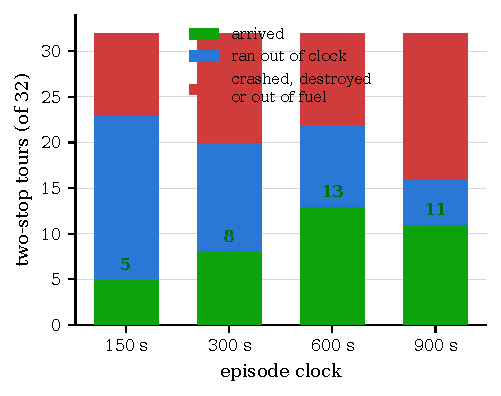
\includegraphics[width=0.46\textwidth]{figures/clock.pdf}
\caption{Thirty-two two-target levels flown by the reference optimizer at
four episode clocks, control resolution held at 3.1\,s per segment. Timeouts
fall monotonically, arrivals peak near 600\,s, and hazard endings rise.}
\label{fig:clock}
\end{figure}

The same experiment on a weaker navigator gives the opposite reading, which
is what makes the pair of measurements informative about the navigator and
not only about the clock. For the present measurement the evaluation suites of
Section~\ref{sec:evaluation} were rebuilt from a
900\,s-validated pool at a 600\,s clock (same families and task
specifications as the 150\,s suites, different levels, so same-family rather
than paired), and the scripted reflex pilot was flown on them: its arrivals
after the 150\,s mark are 1/480, 3/197, 1/47 and 0/136 on the easy, medium,
hard and blind suites, and its 150\,s timeouts (102, 146 and 147 of about
600 on the medium, hard and blind suites) became escapes and collisions at
600\,s rather than arrivals (medium suite: timeouts 102 to 17, escapes 53 to
105, arrivals 206 to 197), an escape being the craft leaving the level past
1.35 times its radius, which a pilot with an empty tank cannot avoid once it
is on an unbound path. A longer clock, that is, gives a navigator the time to
finish a path it could not otherwise finish, or the time to spend its fuel
and drift out, and which of the two it gets depends on the navigator.

The learned policy, trained at a 600\,s clock, is a third case, and the one
that argues most strongly against treating the clock as a free parameter.
Three seeds of the best 150\,s configuration were trained for 3000 updates
with the clock at 600\,s on the long-horizon pool and evaluated on the 600\,s
suites (same families and task specifications as the 150\,s suites, different
levels, so same-family rather than paired; and the blind suite is not blind
at this clock, since no long-horizon pool carries the holdout families). Two
seeds learned and one did not: the two that learned reached 68\% and 74\% on
the easy suite and 26\% and 32\% on the medium suite, against 90\% and 42\%
for the same configuration at 150\,s, while the third never exceeded 19\% on
the easy suite and finished at 4\%, so that the mean over seeds is
$48.9 \pm 38.6$, $19.8 \pm 16.1$, $3.9 \pm 3.6$ and $13.1 \pm 10.5$ on the
four tiers. Note that the dominant ending for the policies that did learn
was still the clock: 37--42\% of medium-suite tasks timed out at 600\,s,
against roughly a third at 150\,s, so that four times the time produced
more timeouts, not fewer. The likely explanation is the discount, since
$\gamma = 0.999$ gives the value estimate a horizon of about 65\,s at
15\,Hz, which is a reasonable fraction of a 150\,s episode and a ninth of a
600\,s one, so that a policy trained at the longer clock is rewarded for
progress it cannot see the end of and is not penalized for drifting. Raising the discount to match the clock confirms this, and
the threshold is sharp. At $\gamma = 0.9995$ (about 133\,s of lookahead) the
failure reproduces almost exactly, with the same seed never learning and
means of $47.7 \pm 38.1$, $20.0 \pm 16.2$, $4.2 \pm 4.1$ and $13.1 \pm 11.1$;
at $\gamma = 0.9998$ (about 333\,s, over half the episode) all three seeds
learn, the seed standard deviations fall to $0.1$--$1.4$ points, and the
policy reaches $83.7 \pm 1.4$, $42.4 \pm 1.4$, $14.1 \pm 0.7$ and
$29.7 \pm 0.1$ on the four tiers, i.e. at or above the 150\,s reference on
medium, hard and blind (on different levels, so same-family rather than
paired, and with the caveat that the 600\,s blind suite is seen-family) and
somewhat below it on easy, with the medium-suite timeout share down from
37--42\% to 26--35\%. Thus, the clock and the discount behave as a single
setting, since a longer clock is available to a learner only together with a
horizon that reaches a substantial fraction of it, and the sense in which
150\,s was arbitrary (Section~\ref{sec:discussion}) does not make 600\,s
correct so much as it makes the pair the quantity that has to be chosen.

The clock cannot simply be set long enough to settle the question, for a
reason that bears on what solvability means. Consider a navigator that does nothing at all. The bodies and a coasting
craft together form an autonomous Hamiltonian system, and on a bounded
energy surface, i.e. one of finite phase-space volume, such a system is
recurrent in the sense Poincar\'e established for exactly this problem
\cite{poincare1890}: almost every trajectory returns arbitrarily close to
its starting state, and so, given enough time, a coasting craft will pass
within the arrival radius of any target it can reach at all, unless an
invariant surface of the kind that survives perturbation in a near-integrable
system \cite{kolmogorov1954,arnold1963} happens to separate it from that
target permanently. Thus, for a flythrough tour, the zero-action policy
succeeds with probability approaching one as the clock lengthens, and the
only stopping criterion that is not a choice is divergence, i.e. the craft
leaving the bounded region; inside it, there is always an improbable path
that has not yet been given time to occur, and in the extreme of a system
that collapses gravitationally toward a point, every path is that path. A
finite clock therefore belongs to the definition of the task, and
solvability is relative to a time budget in the same way that
Section~\ref{sec:eta} makes it relative to a fuel budget, and the question
becomes how much a given navigator's success depends on the allowance. The
same fact is what makes the exhaustive check of Section~\ref{sec:hard}
ill-posed even in principle, since without a horizon the question of whether
a control sequence has failed has no finite answer for a sequence that stays
in the system.

The zero-action navigator was therefore measured directly
(Figure~\ref{fig:noop}). Coasting from the start of every task in the 600\,s
suites for 900\,s (13,500 ticks, the levels' validated horizon), the fraction
of tasks in which the craft passes within the arrival radius of any target
(velocity tolerance and tour order ignored) is 2.3\%, 2.9\%, 5.1\% and 3.7\%
at 150\,s on the easy, medium, hard and blind suites, and 5.3\%, 6.6\%, 9.8\%
and 6.9\% at 900\,s, still rising at the end at about 0.2--0.5 percentage
points per 100\,s; strict completion of the tour as specified by coasting is
0--1.2\% on every tier except easy (5.3\%, where contact is completion). Over
the same interval the fraction of tasks ending in collision, destruction or
escape rises at about 2.5 points per 100\,s on the three harder tiers, to
26--27\% at 900\,s. To see where the contact curve goes, a pool of 900 levels
was validated to 9{,}000\,s (sixty episodes; 80--100\% of generated levels
survive that long, so that the generators' levels remain bounded for at
least that long)
and the same measurement run on it: contact reaches 8.7\%, 9.8\%, 12.9\% and
11.8\% by 9{,}000\,s and is flat over the last 300\,s, because the craft is
dead, with 78--80\% of the non-easy tasks ended by then and destruction by
accumulated damage the commonest ending. Thus, patience alone buys a
coasting craft three to five points of contact between 150\,s and 900\,s and
another three to six between 900\,s and 9{,}000\,s, while over the same
spans the hazard endings rise faster, so that in this environment the
stopping criterion that recurrence fails to supply is supplied by exposure.

\begin{figure}[t]
\centering
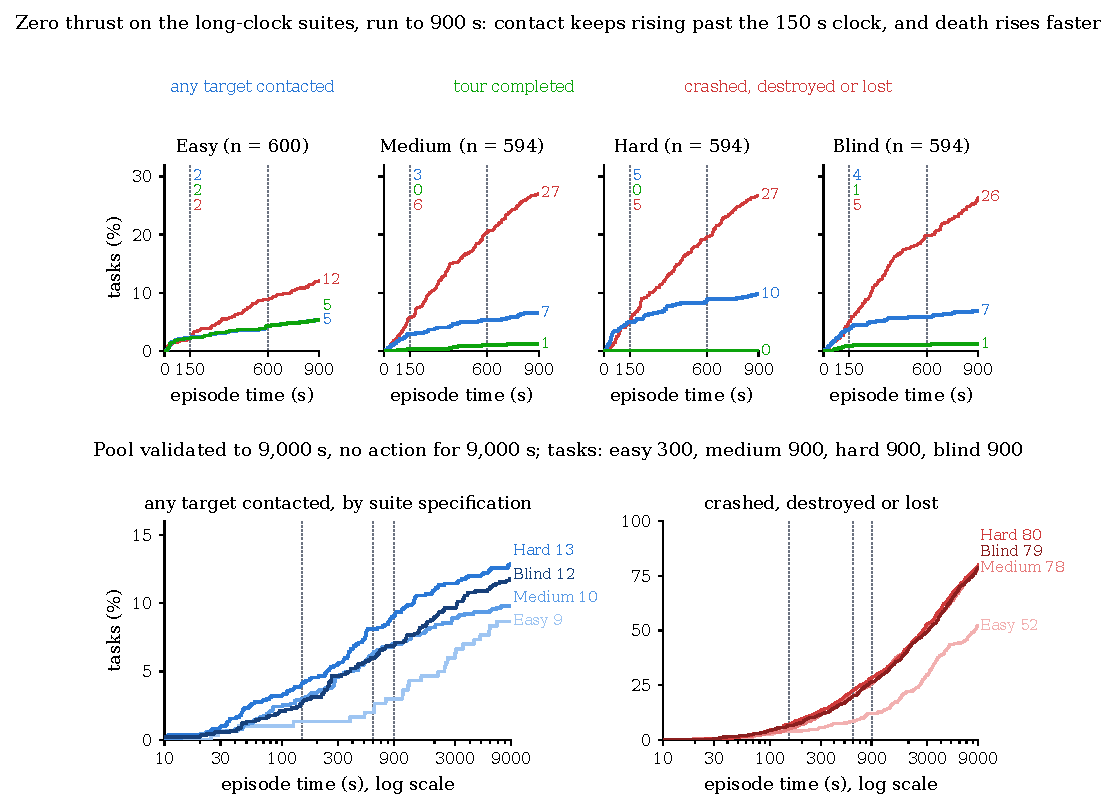
\includegraphics[width=\textwidth]{figures/noop.pdf}
\caption{A craft that never thrusts. Top: on the four 600\,s suites run to
900\,s, the cumulative fraction of tasks in which the craft has passed
within the arrival radius of any target, completed the tour as specified,
or ended in collision, destruction or escape, with rules at the 150\,s clock
and at 600\,s and the values at 150 and 900\,s marked. Bottom: on 900 levels
validated to 9{,}000\,s, the same contact and death curves on a logarithmic
time axis, by suite specification. Computed by \code{scripts/noop\_clock.py};
the two rows are same-specification, not paired.}
\label{fig:noop}
\end{figure}

The expectation that a longer clock matters most on multi-target tasks does
not survive normalization. On the 600\,s suites, a coasting craft first
contacts a target after the 150\,s mark on 2.3\% of single-target and 4.7\%
of multi-target tasks (Fisher's exact $p = 0.001$), but per target slot the
rates are 2.3\% and 2.1\% ($p = 0.81$), and for the first target alone 2.3\%
and 2.2\%; more targets are more chances, and the tour structure adds
nothing. Note that this measurement is on different levels from the 150\,s
suites and is not joined to the agent's per-instance success.
